\chapter{Methodology}
\label{chap:methodology}

\section{Objectives}

The main objective of this experiment is to assess whether RSSI values from ESP32 BLE beacons can reliably determine a smartphone’s position and detect user proximity to a predefined location within a threshold of three meters or less. This validation is crucial for ensuring that the proposed indoor localization system can accurately detect a user's presence near a point of interest (POI).

In addition to the primary objective, secondary goals include evaluating the impact of environmental factors on localization accuracy and analyzing the system’s responsiveness when the user moves dynamically. Furthermore, the study aims to assess how the density of deployed beacons influences the precision of the location estimations. Finally, the experiment will compare localization accuracy across different smartphone models to determine whether variations in hardware affect the system’s performance.

\section{Experimental Setup}

\subsection{Hardware and System Architecture}

The experimental setup comprises up to six ESP32 devices running a custom firmware that enables them to operate as BLE beacons. These devices periodically broadcast BLE signals while simultaneously listening for BLE signals that share a predefined signature. When network access is available, they upload their collected data to an MQTT broker; otherwise, they function solely as standalone BLE beacons. In this phase, the collected values from listening will only be used for offline analysis to determine whether dynamically updating the reference RSSI values could improve precision without directly affecting the experiment.

A smartphone application is responsible for collecting and processing the beacon signals. This application retrieves a list of authorized BLE beacon signatures from the MQTT broker and continuously scans for nearby devices that match these known signatures. No user data is transmitted from the smartphone to the server, ensuring privacy for both the user and other individuals within the area.

\subsection{Application Features and Localization Logic}

The smartphone application provides a real-time graphical interface that visualizes the localization process, primarily for debugging and in-depth analysis. A map displays the static positions of the beacons, with each beacon represented by a circle corresponding to the estimated distance from the phone. Additionally, a dot indicates the estimated position of the smartphone, while crosses mark the predefined points of interest.

Localization is based on RSSI-based triangulation. A phone is considered to be within a POI when it has been detected at least twice within a three-meter radius. Conversely, the phone is considered to have exited the POI if it is subsequently detected twice at a location beyond five meters. This difference between the entry and exit thresholds is implemented to prevent unstable state changes between being inside and outside a POI. These threshold values have been determined based on preliminary evaluations and may be adjusted for different experimental conditions, depending on beacon placement, artwork density, and the complexity of the indoor environment.

\section{Experimental Procedure}

To systematically evaluate the performance of the system, four distinct experiments will be conducted. These experiments focus on evaluating localization accuracy, the impact of beacon density, differences in smartphone models, and system performance during user movement.

\subsection{Experimental Setup}

The experiments will take place in a designated room within the university. ESP32 beacons will be installed at predefined locations to provide adequate coverage of all POIs. The POIs correspond to specific reference points where localization should occur accurately. Participants performing the tests will execute a predefined sequence of movements, ensuring uniformity in data collection and minimizing variability caused by human movement patterns.

Localization data, including timestamps for detected entries, exits, and continuous tracking points, will be logged during all experiments. Additionally, manual records will be kept to compare the system's performance with a ground truth reference, ensuring accurate evaluation.

\subsection{Experiment 1: Localization Accuracy and Responsiveness}

This experiment aims to determine how quickly and reliably the system detects a user entering or exiting a POI and whether position detection remains stable over time.

\begin{enumerate}
    \item The user stands on point $L_2$, outside of the POI area, for one minute.
    \item The user enters the POI (green circle) area at constant speed and stands on point $L_1$, at one meter from its center.
    \item The system records the time required to detect entry and logs the detected position continuously for one minute.
    \item If localization fluctuates, and the user is mistakenly marked as outside the POI, the number and duration of such misclassifications are recorded.
    \item The user exits the POI (red circle) at constant speed, and the system logs the delay before detecting the exit.
\end{enumerate}

\begin{figure}[H]
    \centering
    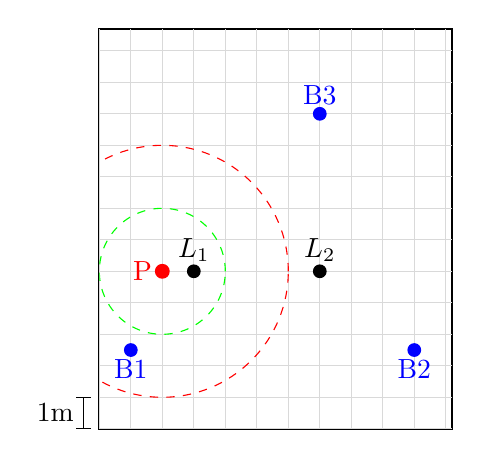
\begin{tikzpicture}[scale=0.4]
        % Room dimensions 
        \draw[thick] (0,0) rectangle (11.2,12.7);  
        % Grid (optional, for reference)
        \draw[gray!30, step=1] (0,0) grid (11.2,12.7);
        
        % ESP32 devices (blue dots)
        \filldraw[blue] (1,2.5) circle (0.2) node[below] {B1};
        \filldraw[blue] (10,2.5) circle (0.2) node[below] {B2};
        \filldraw[blue] (7,10) circle (0.2) node[above] {B3};
        
        % Point of Interest (red cross)
        \filldraw[red, thick] (2,5) circle (0.2) node[left] {P};

        % User positions (X marks)
        \filldraw (3,5) circle (0.2) node[above] {$L_1$};
        \filldraw (7,5) circle (0.2) node[above] {$L_2$};
            
        \begin{scope}
            \clip (0,0) rectangle (11.2,12.7);
            % 3m radius around POI (dashed circle)
            \draw[red, dashed] (2,5) circle (4);
            \draw[green, dashed] (2,5) circle (2);
        \end{scope}
        
        % Scale indicator
        \draw[|-|] (-0.5,0) -- (-0.5,1) node[midway, left] {1m};
    \end{tikzpicture}
    \caption{Experimental setup for the first experiment showing three ESP32 devices and a single POI with its detection radius.}
    \label{fig:exp1_setup}
\end{figure}

\subsection{Experiment 2: Impact of Beacon Density}
This experiment evaluates how the number of deployed ESP32 beacons affects localization accuracy by progressively adding beacons to the setup while maintaining the same test procedure.
\begin{enumerate}
    \item Steps from Experiment 1 are repeated for this configuration, but a fourth beacon (B4) is added and the test is repeated.
    \item A fifth beacon (B5) is added and the test is repeated.
    \item Finally, a sixth beacon (B6) is added completing the test series.
\end{enumerate}

\begin{figure}[H]
    \centering
    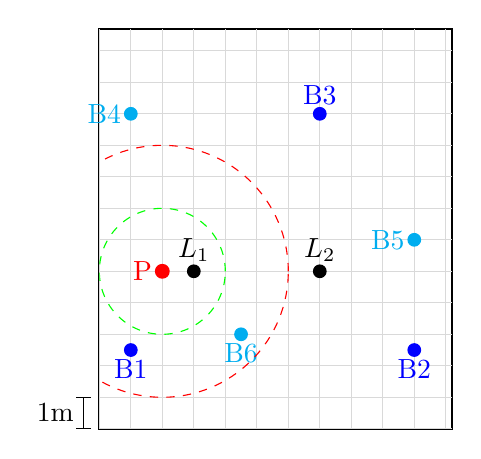
\begin{tikzpicture}[scale=0.4]
        % Room dimensions
        \draw[thick] (0,0) rectangle (11.2,12.7);  
        % Grid (optional, for reference)
        \draw[gray!30, step=1] (0,0) grid (11.2,12.7);
        % Original ESP32 devices (blue dots)
        \filldraw[blue] (1,2.5) circle (0.2) node[below] {B1};
        \filldraw[blue] (10,2.5) circle (0.2) node[below] {B2};
        \filldraw[blue] (7,10) circle (0.2) node[above] {B3};
        % Additional beacons (different color)
        \filldraw[cyan] (1,10) circle (0.2) node[left] {B4};
        \filldraw[cyan] (10,6) circle (0.2) node[left] {B5};
        \filldraw[cyan] (4.5,3) circle (0.2) node[below] {B6};
        % Point of Interest (red cross)
        \filldraw[red, thick] (2,5) circle (0.2) node[left] {P};
        % User positions (X marks)
        \filldraw (3,5) circle (0.2) node[above] {$L_1$};
        \filldraw (7,5) circle (0.2) node[above] {$L_2$};
        \begin{scope}
            \clip (0,0) rectangle (11.2,12.7);
            % 3m radius around POI (dashed circle)
            \draw[red, dashed] (2,5) circle (4);
            \draw[green, dashed] (2,5) circle (2);
        \end{scope}
        % Scale indicator
        \draw[|-|] (-0.5,0) -- (-0.5,1) node[midway, left] {1m};
    \end{tikzpicture}
    \caption{Experimental setup showing all six ESP32 devices, with B4-B6 representing the additional beacons for density testing.}
    \label{fig:exp2_setup}
\end{figure}

\subsection{Experiment 3: Effect of Smartphone Models}
This experiment investigates whether localization accuracy varies across different Android smartphone models using the maximum beacon density configuration.
\begin{enumerate}
    \item The complete procedure from Experiment 1 is performed using each test device.
    \item Results are compared across devices to evaluate hardware-dependent variations.
\end{enumerate}

\subsection{Experiment 4: Impact of Dynamic Movement}
This experiment evaluates the system's ability to track a moving user between multiple POIs.
\begin{enumerate}
    \item Using the three-beacon configuration, two additional POIs are added to the setup.
    \item The user starts at $L_2$ and walks at a constant pace toward $L_1$.
    \item After one minute at $L_1$, the user moves to $L_3$ and stand for one minute.
    \item After one minute at $L_3$, the user moves to $L_4$ and stand for one minute.
    \item The system logs transition times and tracking consistency throughout the movement.
\end{enumerate}

\begin{figure}[H]
    \centering
    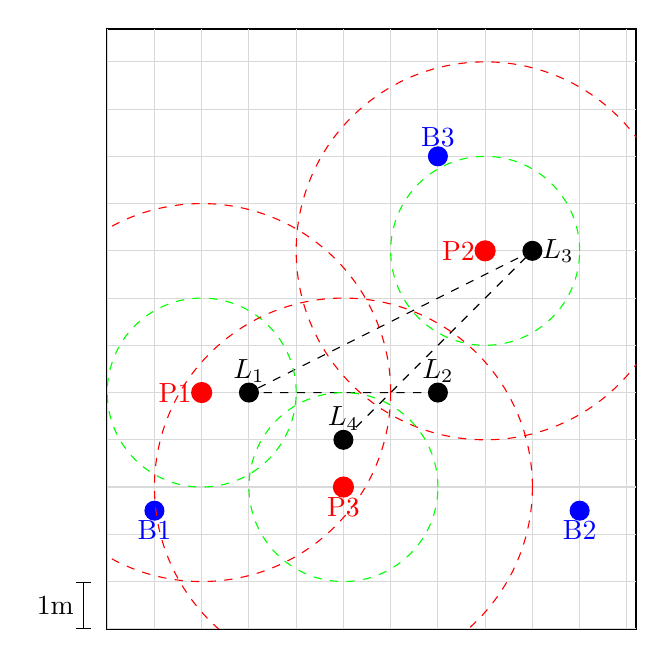
\begin{tikzpicture}[scale=0.6]
        % Room dimensions
        \draw[thick] (0,0) rectangle (11.2,12.7);  
        % Grid (optional, for reference)
        \draw[gray!30, step=1] (0,0) grid (11.2,12.7);
        % All ESP32 devices
        \filldraw[blue] (1,2.5) circle (0.2) node[below] {B1};
        \filldraw[blue] (10,2.5) circle (0.2) node[below] {B2};
        \filldraw[blue] (7,10) circle (0.2) node[above] {B3};
        % Multiple POIs
        \filldraw[red, thick] (2,5) circle (0.2) node[left] {P1};
        \filldraw[red, thick] (8,8) circle (0.2) node[left] {P2};
        \filldraw[red, thick] (5,3) circle (0.2) node[below] {P3};
        % User positions and path
        \filldraw (3,5) circle (0.2) node[above] {$L_1$};
        \filldraw (7,5) circle (0.2) node[above] {$L_2$};
        \filldraw (9,8) circle (0.2) node[right] {$L_3$};
        \filldraw (5,4) circle (0.2) node[above] {$L_4$};
        % Movement path
        \draw[->, dashed] (7,5) -- (3,5) -- (9,8) -- (5,4);
        \begin{scope}
            \clip (0,0) rectangle (11.2,12.7);
            % Detection radii around POIs
            \draw[red, dashed] (2,5) circle (4);
            \draw[green, dashed] (2,5) circle (2);
            \draw[red, dashed] (8,8) circle (4);
            \draw[green, dashed] (8,8) circle (2);
            \draw[red, dashed] (5,3) circle (4);
            \draw[green, dashed] (5,3) circle (2);
        \end{scope}
        % Scale indicator
        \draw[|-|] (-0.5,0) -- (-0.5,1) node[midway, left] {1m};
    \end{tikzpicture}
    \caption{Experimental setup for dynamic movement testing, showing all beacons, multiple POIs, and the user movement path.}
    \label{fig:exp4_setup}
\end{figure}